Más especificamente, \textcolor{red}{estimamos un RTT medio} para cada salto que
se da en la ruta que nos comunica con cada host, y \textcolor{red}{normalizamos
este valor para conseguir el Z-score de los RTT (ZRTT)} para cada salto que nos
de suficiente informaci\'on como para \textcolor{red}{analizar el trasfondo del
tr\'afico en la red}.

\begin{figure}[!h]
  \begin{center}
      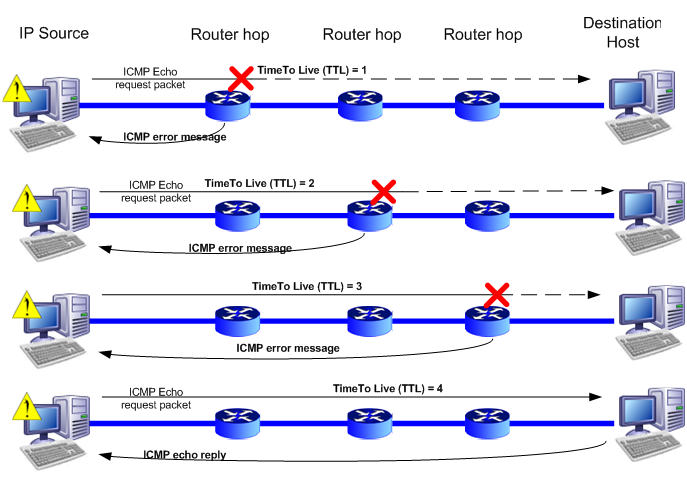
\includegraphics[scale=0.4]{imagenes/traceroute.png}
      \caption{Mecanismo de acción de traceroute}
      \label{fig:contra1}
  \end{center}
\end{figure}

Para analizar las rutas que pueden pasar por cables submarinos, hicimos este
an\'alisis a cuatro universidades:

\begin{itemize}
	\item [MSU] {\foreignlanguage{russian}{Московский государственный
	университет имени М. В. Ломоносова}
	(Universidad Estatal de Mosc\'u) Federaci\'on Rusa}
	\item [Oxford] {University of Oxford, Reino Unido}
	\item [Queensland] {University of Queensland, Australia}
	\item [Tsinghua] {\foreignlanguage{chinese}{清华大学} (Universidad de Tsinghua), China}
\end{itemize}

Por cada host, se env\'ian 10 paquetes con \textit{Time to Live} diferente hasta
llegar al host indicado, y se toma la media estad\'istica de el \textit{Round
Trip Time} de cada tramo.

Hay muchos hosts donde la acci\'on de responder paquetes ICMP se le da
much\'isima menor prioridad que la acci\'on de forwardearlos a otro host. Por
esta raz\'on hay muchos hosts que dan un \textit{Round Trip Time} mayor a otro
host a pesar de ser m\'as ``cercanos'' en la red y fisicamente al cliente.
Aunque en la mayor\'ia de los hosts esto no cambia mucho nuestros resultados (ya que
solo queremos buscar links continentales), hay algunos hosts donde la diferencia
entre RTT dado y el real es demasiado alta. Por esta raz\'on solo tomamos
paquetes con un RTT menor a \textbf{1 segundo}, e ignoramos los hosts donde
todos los 10 paquetes fueron ignorados.
